\chapter{Methodology and Concept Development}
\label{chap:methodology}

This chapter presents the systematic approach taken in designing the \ac{VMAP} system. The methodology follows established software engineering principles to address the complex requirements of automotive parameter management. Beginning with a requirements analysis, the chapter proceeds to detail the conceptual architecture design, data model, validation mechanisms, and integration approaches developed to ensure system robustness and compatibility with existing enterprise infrastructure.

\section{Requirements Analysis}
\label{sec:requirements-analysis}

The foundation of the \ac{VMAP} system design was a comprehensive requirements \mbox{analysis} conducted through a series of structured interviews with stakeholders, detailed examination of the existing Excel-based process, and workshops with domain experts. This multi-faceted approach, following Sommerville's framework for requirements engineering, ensured that both functional and non-functional requirements would be thoroughly identified and prioritized \cite{sommerville2011software}.

\subsection{Functional Requirements}
\label{subsec:functional-requirements}

The primary functional requirements were derived from direct observation of engineers' current Excel-based workflow combined with semi-structured interviews conducted with module developers and documentation specialists. Through this process, several critical requirements emerged for the \ac{VMAP} system.

The system must support the hierarchical organization of parameters within \acp{ECU}, Modules, and \acp{PID}, mirroring the domain-specific structure of automotive electronic systems as described by Staron \cite{staron2021automotive}. This hierarchical organization is essential for maintaining the logical structure of vehicle parameters and aligning with established engineering practices.

Users must be able to create variants for parameters with specific code rules determining their applicability, and define segments representing modified parameter values. If no segment exists, the system must default to Parameter Definition Database values—an approach that allows efficient storage by tracking only modifications rather than duplicating unchanged parameters, aligning with Bhattacherjee's principles of dataset versioning \cite{bhattacherjee2015principles}.

The system must track parameter values across four distinct release phases: Phase1, Phase2, Phase3, and Phase4, with changes in earlier phases propagating to later phases unless explicitly overridden. This phase-based approach represents a domain-specific adaptation particularly suited to automotive software development cycles as identified in Broy's research on automotive software engineering challenges \cite{broy2006challenges}.

All modifications require comprehensive logging with user information, timestamp, and detailed change data, supporting regulatory compliance and enabling parameter evolution tracking. Through the stakeholder interviews, it was determined that the system must also provide functionality to create parameter configuration snapshots at specific points, particularly at phase transitions, for documentation purposes—a capability identified as essential for quality assurance and regulatory compliance in automotive software development by Staron \cite{staron2021automotive}.

\subsection{Integration with External Systems}
\label{subsec:integration-external-systems}

The stakeholder interviews and process analysis revealed that \ac{VMAP} must integrate with two critical external enterprise systems: the \ac{PDD} and the \ac{VCD}.

The \ac{PDD} serves as the authoritative source for the hierarchical structure of automotive electronic systems, containing definitions of \acp{ECU}, Modules, \acp{PID}, and baseline parameter configurations. As noted by Pretschner et al. \cite{pretschner2007software}, maintaining this hierarchical structure is essential for automotive software development. The workshops with domain experts confirmed that while \ac{VMAP} will manage parameter variants and customizations, it must rely on \ac{PDD} for the underlying parameter definitions and structural relationships, requiring a robust synchronization mechanism to maintain consistency between the systems.

The \ac{VCD} contains comprehensive vehicle specifications and configuration codes that determine which parameter variants apply to specific vehicle configurations. Integration with this system is necessary for two critical functions: validating the boolean code rules associated with parameter variants to ensure they reference valid vehicle codes, and supporting parameter file generation for specific vehicle configurations by resolving the applicable parameter variants based on vehicle codes. This integration requirement aligns with Staron's analysis of automotive software architectures, which emphasizes the importance of configuration management in supporting variant-rich vehicle platforms \cite{staron2021automotive}.

These integration requirements necessitated careful consideration of data synchronization approaches, leading to an exploration of different strategies for maintaining consistency between \ac{VMAP} and these external systems while minimizing performance impact and complexity.

\subsection{User Role Requirements}
\label{subsec:user-role-requirements}

A systematic analysis of the current Excel-based workflow, coupled with contextual inquiries with engineering teams, identified four distinct user roles with specific access requirements. This analysis included shadowing users in their daily work, documenting their tasks and access patterns, and conducting structured interviews to validate the observed patterns.

Module developers require write access to parameters within their assigned modules, with the ability to create and modify variants and segments. Documentation specialists need access to frozen data for documentation, comparison capabilities between phases, and comprehensive change history access. System administrators require comprehensive control over user management, release phases, and special operations like variant deletion and phase freezing. Read-only users need view access to all parameter data with parameter file generation capabilities but no modification rights.

These roles were defined based on the principle of least privilege as described by Sandhu \cite{sandhu1998role}, ensuring users have access only to functionality required for their specific responsibilities. This enhances system security while simplifying the user experience by presenting only relevant options.

\subsection{Data Management Requirements}
\label{subsec:data-management-requirements}

The system must maintain distinct parameter versions across different release phases, allowing simultaneous work on multiple phases while enabling access to parameter values from any point in the development lifecycle. As highlighted by Elmasri and Navathe \cite{elmasri2015fundamentals}, data integrity requires maintaining referential integrity across all related entities, particularly ensuring variants and segments associate with valid parameters.

Multi-dimensional parameter support is essential for complex automotive parameters such as mapping tables. Operations modifying multiple related entities must function as atomic transactions to maintain data consistency—particularly important for phase transitions where numerous parameters, variants, and segments may change simultaneously, a requirement that aligns with Bhattacherjee's research on dataset versioning approaches \cite{bhattacherjee2015principles}.

Query performance analysis, based on projected usage patterns from the current Excel-based process, identified critical query paths including parameter retrieval by \ac{ECU}, module, \ac{PID}, release phase, and parameter name. These requirements influenced schema design decisions regarding normalization and indexing strategies to optimize common query patterns.

\section{Use Case Modeling}
\label{sec:use-case-modeling}

Following the requirements gathering process, use case modeling was employed to formalize the system's functional requirements from a user perspective. This approach, as described by Jacobson \cite{jacobson2004use}, provides a structured way to represent the system's capabilities and the interactions between users and the system.

\begin{figure}[h]
    \centering
    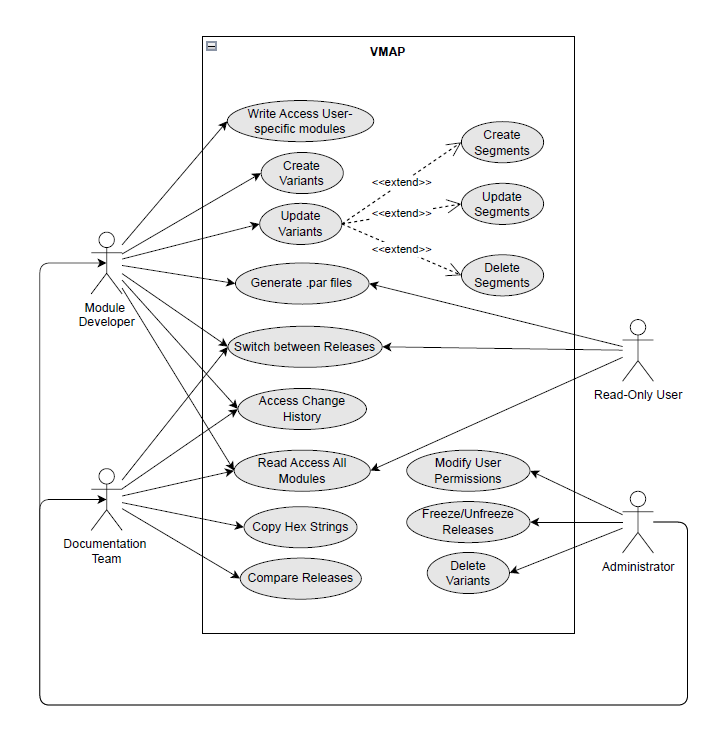
\includegraphics[width=0.95\textwidth]{figures/vmap_use_case_diagram.png}
    \caption{\ac{VMAP} System Use Case Diagram}
    \label{fig:use-case-diagram}
\end{figure}

The use case diagram in Figure \ref{fig:use-case-diagram} illustrates the primary actors and their interactions with the \ac{VMAP} system. Four primary actor types are identified, corresponding to the user roles established during requirements analysis: Module Developers, who create and modify parameter variants; Documentation Team members, who access parameter data for documentation purposes; Administrators, who manage system settings and user access; and Read-Only Users, who view parameter data without making modifications.

The diagram demonstrates how these actors interact with key system functionalities. Module Developers primarily interact with variant creation and modification use cases, while having limited access to parameter viewing and comparison features. Documentation Team members focus on viewing frozen configurations, comparing parameters across phases, and accessing change history. Administrators have access to all system functions, including user management, release configuration, and system settings. Read-Only Users are limited to viewing parameters and generating parameter files.

This use case model provides a clear visual representation of the system's scope and functionality, serving as a bridge between user requirements and technical implementation. By mapping user roles to specific system functions, the model ensures that the database design will support all required user interactions while maintaining appropriate access controls.

\section{User Management Approaches}
\label{sec:user-management-approaches}

Based on the identified user role requirements, two distinct approaches to user management were considered for the \ac{VMAP} system: a traditional role-based approach and a hybrid role-permission approach. Each approach offers different advantages in terms of flexibility, administrative complexity, and alignment with organizational needs.

\subsection{Traditional Role-Based Approach}
\label{subsec:traditional-role-approach}

\begin{figure}[h]
    \centering
    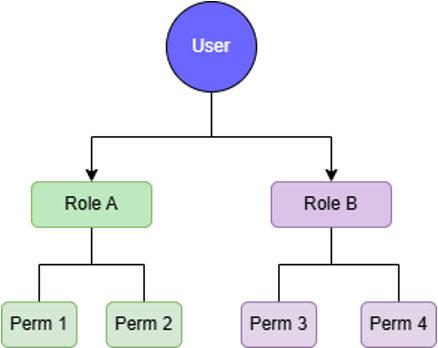
\includegraphics[width=0.7\textwidth]{figures/traditional_rbac_model.png}
    \caption{Traditional Role-Based Access Control Approach}
    \label{fig:traditional-rbac}
\end{figure}

The traditional role-based approach, illustrated in Figure \ref{fig:traditional-rbac}, assigns users to predefined roles that contain fixed sets of permissions, following the classic \ac{RBAC} model described by Sandhu \cite{sandhu1998role}. In this approach, each user is assigned one or more roles (Administrator, Module Developer, Documentation Team, Read-Only User), and all permissions are granted through these role assignments without individual permission adjustments.

This approach offers administrative simplicity, as user management involves only assigning appropriate roles rather than configuring individual permissions. The role structure also provides clear organizational alignment, with roles directly corresponding to job functions within the development process. From an implementation perspective, this approach simplifies permission checking, typically requiring only verification of role membership rather than individual permission verification.

A key limitation of this approach is its reduced flexibility for accommodating exceptions or specialized access requirements. If a user requires a subset of permissions that doesn't align with existing roles, administrators must either create a new role specifically for that user or grant a role with more permissions than strictly necessary, potentially compromising the principle of least privilege \cite{sandhu1998role}.

\subsection{Hybrid Role-Permission Approach}
\label{subsec:hybrid-approach}

\begin{figure}[h]
    \centering
    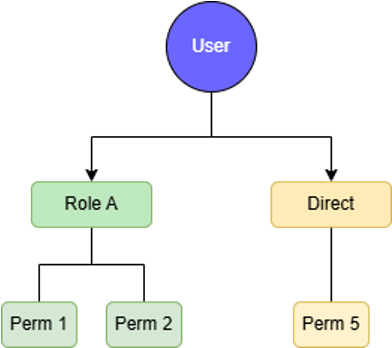
\includegraphics[width=0.7\textwidth]{figures/hybrid_rbac_model.png}
    \caption{Hybrid Role-Permission Access Control Approach}
    \label{fig:hybrid-rbac}
\end{figure}

The hybrid approach, illustrated in Figure \ref{fig:hybrid-rbac}, combines role-based permissions with direct permission assignments, similar to the model described by Ferraiolo et al. \cite{ferraiolo2011policy}. In this approach, users are assigned to primary roles defining their core permissions, but additional permissions can be granted on a per-user basis to address exceptional cases or specialized responsibilities.

This approach offers greater flexibility for accommodating exceptions without creating specialized roles, essential in environments where organizational structures evolve over time. It provides more granular permission control, allowing precise tailoring of access rights to individual responsibilities. However, this flexibility comes at the cost of increased administrative complexity, as both roles and individual permissions must be managed.

The hybrid approach is particularly valuable in the automotive parameter management context, where development responsibilities can vary between projects and temporary access adjustments may be needed for specific tasks or during transition periods. The approach balances structured role assignments with the flexibility to accommodate evolving access requirements, a common scenario in complex engineering environments like automotive development.

\section{Parameter Synchronization Approaches}
\label{sec:parameter-sync-approaches}

Integration with the \ac{PDD} represents a critical aspect of the \ac{VMAP} system, requiring careful consideration of synchronization approaches. Two different conceptual approaches were explored for maintaining parameter data across the release phases: the change-based approach and the phase-based approach.

\subsection{Change-Based Synchronization Approach}
\label{subsec:change-based-sync}

\begin{figure}[h]
    \centering
    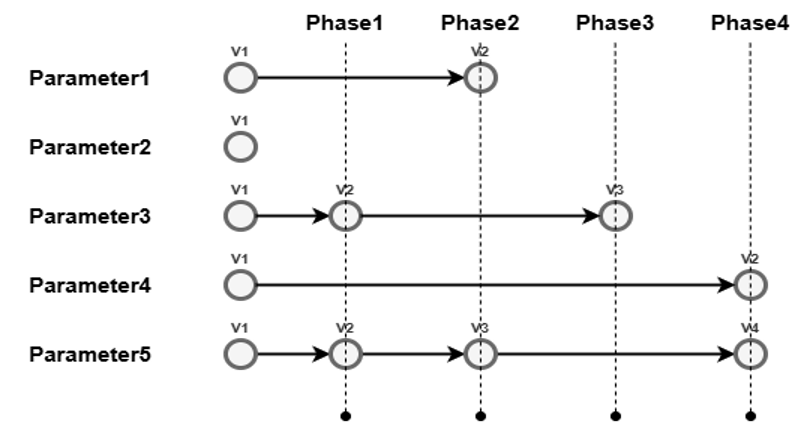
\includegraphics[width=0.95\textwidth]{figures/change_based_approach.png}
    \caption{Change-Based Parameter Synchronization Approach}
    \label{fig:change-based-sync}
\end{figure}

The change-based approach, illustrated in Figure \ref{fig:change-based-sync}, maintains parameter values by recording changes between phases rather than storing complete parameter sets for each phase. In this model, parameters are initially created before the first phase (Phase1), and subsequent modifications are recorded as change entries associated with specific phases.

When a parameter changes in a later phase (like Phase2), only the specific change is recorded rather than creating a new complete copy of the parameter. As shown in the figure, Parameter1 is created before Phase1 with version V1, then modified in Phase2 (creating version V2), but remains unchanged in Phase3 and Phase4. Similarly, Parameter3 changes in Phase1 and Phase3, while Parameter5 changes in every phase except Phase3.

This approach is conceptually aligned with traditional version control systems as described by Bhattacherjee et al. \cite{bhattacherjee2015principles}, where efficiency is achieved by storing only the differences between versions rather than complete copies. The approach potentially offers storage efficiency advantages by minimizing data duplication across phases, which could be significant for parameter sets containing thousands of entries.

However, this approach introduces conceptual complexity for retrieving parameter values in a specific phase. To determine a parameter's value for a given phase, the system must identify the most recent version of that parameter up to and including the target phase. This reconstruction process introduces additional processing steps compared to direct parameter retrieval.

\subsection{Phase-Based Synchronization Approach}
\label{subsec:phase-based-sync}

\begin{figure}[h]
    \centering
    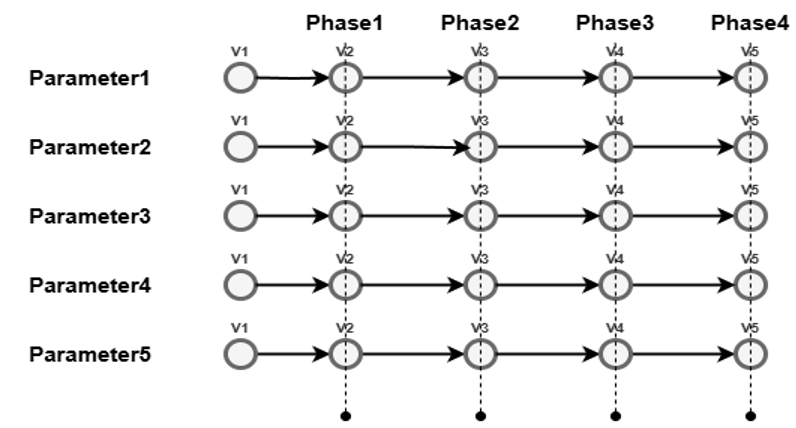
\includegraphics[width=0.95\textwidth]{figures/phase_based_approach.png}
    \caption{Phase-Based Parameter Synchronization Approach}
    \label{fig:phase-based-sync}
\end{figure}

The phase-based approach, illustrated in Figure \ref{fig:phase-based-sync}, maintains complete parameter sets for each phase independently. When parameters are initially created before Phase1, each parameter has its specific version (V1). When transitioning to a new phase, all parameters are copied forward, even if they haven't changed. If a parameter is subsequently modified in the new phase, it receives a new version specific to that phase.

As shown in the figure, each parameter exists in every phase with a phase-specific version, regardless of whether the parameter value actually changed between phases. This creates a clear separation between phases, with each phase maintaining its complete parameter configuration independently.

This approach aligns more directly with the phase-oriented structure of automotive development described by Broy \cite{broy2006challenges}, where distinct development milestones form the primary organizational principle. The approach simplifies conceptual understanding and parameter retrieval, as parameters for a specific phase can be accessed directly without reconstructing their values from change history.

The phase-based approach also simplifies phase inheritance by copying parameter configurations forward during phase transitions, allowing subsequent modifications in each phase without affecting previous phases. This copying mechanism preserves the integrity of phase data while supporting the automotive development process, where configurations stabilize progressively through successive phases.

The primary consideration with this approach is the increased storage requirements, as parameters are duplicated across phases even when they haven't changed. However, this trade-off potentially provides benefits in terms of conceptual clarity, query simplicity, and alignment with the automotive development workflow.

\section{Database System Considerations}
\label{sec:database-system-considerations}

Selecting an appropriate database management system for \ac{VMAP} required consideration of different options against the specific requirements of automotive parameter management. Four major relational database systems were considered as potential platforms for the \ac{VMAP} implementation: PostgreSQL, Oracle, Microsoft SQL Server, and MySQL.

\subsection{Database System Requirements}
\label{subsec:database-requirements}

The requirements analysis identified several critical database capabilities needed for effective parameter management. First, support for complex data types, including arrays for multi-dimensional parameters and structured types for variant definitions, is essential for representing the sophisticated parameter structures common in automotive systems. Second, robust transaction support for maintaining data consistency during operations affecting multiple related entities ensures data integrity during complex operations such as phase transitions. Third, advanced indexing capabilities are required to optimize the performance of common query patterns, particularly parameter retrieval across different dimensions of the hierarchical structure. Fourth, extensibility for implementing domain-specific operations and validation rules enables the system to incorporate automotive-specific logic directly within the database layer. Fifth, comprehensive access control mechanisms supporting the role-based security model are necessary for managing user permissions across different organizational roles. Finally, efficient storage and retrieval of historical data for audit and traceability purposes supports both regulatory compliance and diagnostic capabilities.

These requirements guided the evaluation of different database systems, focusing on their respective strengths and limitations in addressing the specific needs of automotive parameter management.

\subsection{Comparative Analysis of Database Systems}
\label{subsec:database-comparison}

Table \ref{tab:database-comparison} presents a comparative analysis of the four database systems considered for the \ac{VMAP} implementation, evaluating each against criteria relevant to automotive parameter management.

\begin{table}[htbp]
\centering
\caption{Comparison of Database Systems for Automotive Parameter Management}
\label{tab:database-comparison}
\begin{tabular}{|p{2.5cm}|p{2.5cm}|p{2.5cm}|p{2.5cm}|p{2.5cm}|}
\hline
\textbf{Feature} & \textbf{PostgreSQL} & \textbf{Oracle} & \textbf{SQL Server} & \textbf{MySQL} \\
\hline
\textbf{Complex Data Types} & 
Excellent support for arrays, JSON, custom types \cite{obe2017postgresql} & 
Good support, additional licensing for advanced features \cite{agarwaloracle} & 
Limited built-in support, extensions required \cite{ben2017mcsa} & 
Limited support, improved in recent versions \cite{williams2004web} \\
\hline
\textbf{Transaction Support} & 
Comprehensive with serializable isolation \cite{obe2017postgresql} & 
Excellent with advanced options \cite{agarwaloracle} & 
Robust support with multiple isolation levels \cite{ben2017mcsa} & 
Limited in some storage engines \cite{schwartz2012high} \\
\hline
\textbf{Indexing Capabilities} & 
Diverse index types including GIN for text search \cite{obe2017postgresql} & 
Advanced indexing with optimizer hints \cite{agarwaloracle} & 
Solid capabilities with columnstore indexes \cite{ben2017mcsa} & 
Basic indexing with some limitations \cite{schwartz2012high} \\
\hline
\textbf{Extensibility} & 
Highly extensible with custom types and functions \cite{obe2017postgresql} & 
Extensible with proprietary mechanisms \cite{agarwaloracle} & 
Extensible through .NET integration \cite{ben2017mcsa} & 
Limited extensibility \cite{williams2004web} \\
\hline
\textbf{Access Control} & 
Fine-grained with role-based mechanisms \cite{obe2017postgresql} & 
Comprehensive with advanced security features \cite{agarwaloracle} & 
Strong integration with Active Directory \cite{ben2017mcsa} & 
Basic capabilities with plugin architecture \cite{williams2004web} \\
\hline
\textbf{Licensing} & 
Open source, PostgreSQL License \cite{obe2017postgresql} & 
Commercial, complex licensing model \cite{agarwaloracle} & 
Commercial with edition-based pricing \cite{ben2017mcsa} & 
Dual licensing: GPL and commercial \cite{williams2004web} \\
\hline
\end{tabular}
\end{table}

The comparative analysis revealed different strengths among the database systems. PostgreSQL offers excellent support for complex data types and extensibility, particularly valuable for representing multi-dimensional parameters and implementing domain-specific operations. Oracle provides robust enterprise features with sophisticated optimization capabilities but introduces licensing complexity. SQL Server offers strong integration with Microsoft technologies, while MySQL provides simplicity but has limitations for complex data management requirements.

\subsection{Database System Selection}
\label{subsec:database-system-selection}

Based on the comparative analysis, PostgreSQL was selected as the database platform for the \ac{VMAP} implementation. This decision was driven by several key factors that align with the specific requirements of automotive parameter management. PostgreSQL's native support for arrays, JSON/JSONB, and custom data types provides essential capabilities for representing multi-dimensional parameters and complex variant structures. This eliminates the need for complex workarounds or additional middleware components that would be required with other database systems \cite{obe2017postgresql}. The ability to create custom functions, data types, and operators in PostgreSQL enables implementation of domain-specific operations directly within the database. This capability is particularly valuable for implementing parameter resolution algorithms and validation logic that can execute efficiently at the database level \cite{obe2017postgresql}.

PostgreSQL's diverse indexing capabilities, including GIN indexes for full-text search and partial indexes for conditional indexing, provide optimal support for the complex query patterns common in parameter management. These capabilities are essential for maintaining performance with the large parameter datasets typical in automotive applications \cite{obe2017postgresql}. PostgreSQL's implementation of MVCC (Multi-Version Concurrency Control) and support for various isolation levels ensures data consistency during complex operations affecting multiple related entities, which is critical for maintaining parameter integrity during phase transitions and bulk operations \cite{obe2017postgresql}.

The open-source nature of PostgreSQL eliminates licensing costs while providing enterprise-grade capabilities. This factor was particularly important for the research context of this thesis, enabling implementation without commercial licensing constraints. PostgreSQL's vibrant development community and regular release cycle provide assurance of continued innovation and support, which is important for long-term system sustainability \cite{obe2017postgresql}.

While Oracle provides comparable technical capabilities and would be suitable for enterprise deployment, its complex licensing model and higher total cost of ownership make it less appropriate for this research implementation. Similarly, while SQL Server offers robust enterprise features, its Windows-centric approach and licensing requirements present unnecessary constraints for this application. MySQL, despite its popularity and simplicity, lacks several advanced features required for sophisticated parameter management, particularly in areas of complex data types, extensibility, and advanced indexing capabilities \cite{williams2004web}.

The selection of PostgreSQL provides a solid foundation for implementing the sophisticated database features required by the \ac{VMAP} system while maintaining the flexibility needed for research and development activities.

\section{Entity-Relationship Model}
\label{sec:entity-relationship-model}

Based on the requirements analysis and architectural considerations, a comprehensive \ac{ER} model was developed to capture the complex relationships between system entities. This model follows the approach described by Chen \cite{chen1976entity}, providing a conceptual foundation for the database implementation.

\begin{figure}[h]
\centering
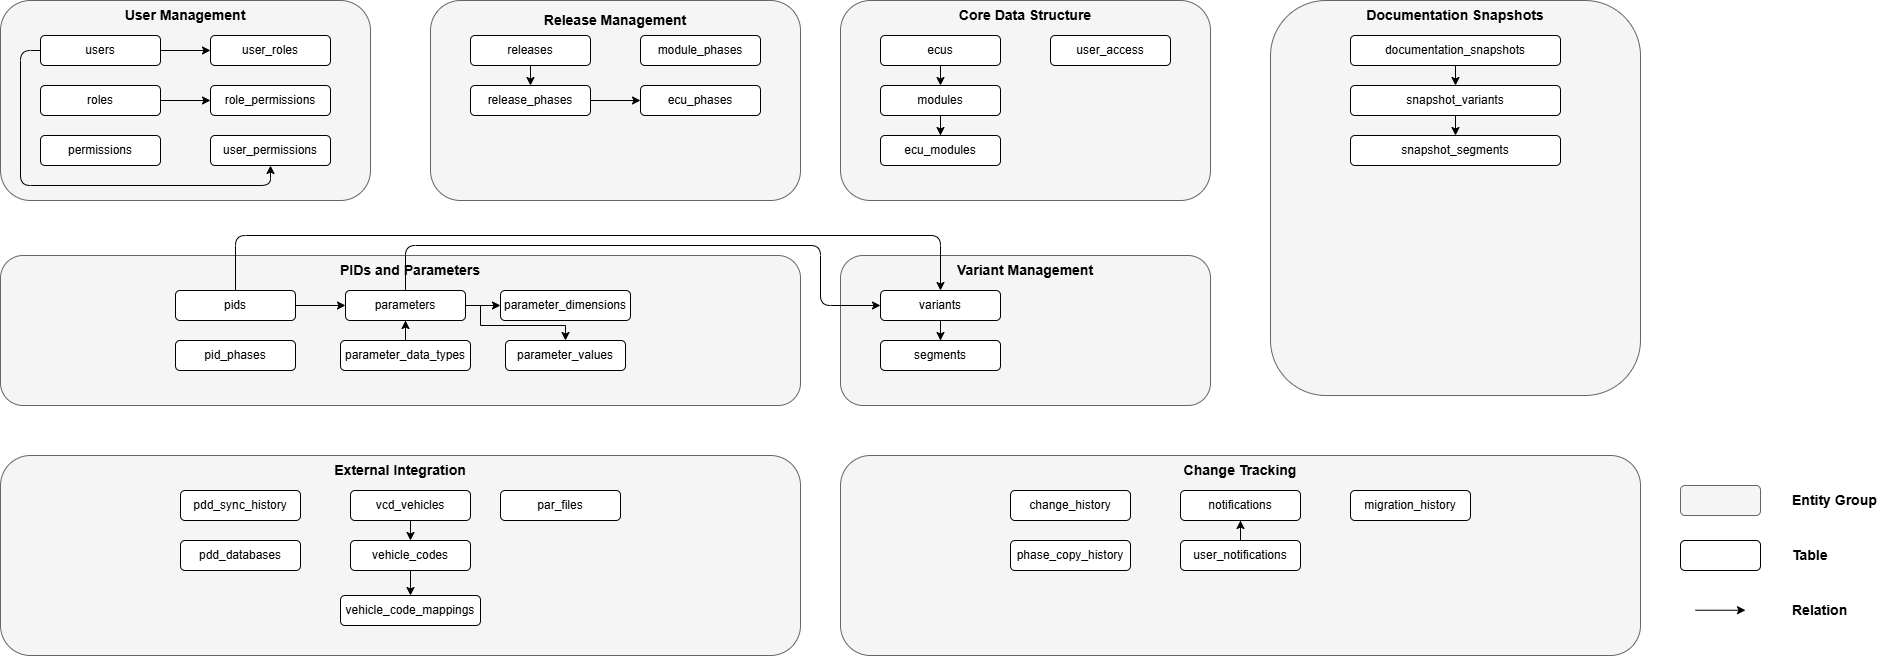
\includegraphics[width=1.0\textwidth]{figures/vmap_er_diagram.png}
\caption{Comprehensive Entity-Relationship Diagram for the \ac{VMAP} System}
\label{fig}
\end{figure}
Figure \ref{fig} illustrates the complete entity-relationship model for the \ac{VMAP} system, showing the logical organization of entities into functional groups and the relationships between them. The diagram captures the hierarchical structure of automotive parameter data, the phase-based versioning approach, the role-permission access control model, and the mechanisms for external system integration and change tracking.

\subsection{Core Data Entities}
\label{subsec:core-data-entities}

The \ac{ER} model includes several categories of entities representing different aspects of the system:

User management entities include Users, Roles, Permissions, and their relationships, implementing a role-permission model for access control. These entities support the authentication and authorization requirements identified during the requirements analysis.

Release management entities encompass Releases, Release Phases, and \ac{ECU} Phase mappings, providing the foundation for the phase-based version control approach. These entities support the automotive development cycle with its distinct phases and milestones.

Parameter structure entities include \acp{ECU}, Modules, \acp{PID}, Parameters, and Parameter Dimensions, representing the hierarchical organization of vehicle electronic systems as described by Staron \cite{staron2021automotive}. These entities capture both the structure and characteristics of parameters, including multi-dimensional parameters like maps and tables.

Variant management entities comprise Variants, Segments, and their relationships to parameters, implementing the core parameter customization functionality. These entities support the creation of parameter variations for different vehicle configurations and operating conditions.

Documentation entities include Documentation Snapshots, Snapshot Variants, and Snapshot Segments, supporting the preservation of historical parameter states for documentation and regulatory compliance. These entities enable the creation of complete parameter configuration snapshots at specific development milestones.

Integration entities consist of Synchronization Records, Vehicle Configurations, and Parameter File Records, supporting connectivity with the Parameter Definition Database and Vehicle Configuration Database. These entities track synchronization operations and store the necessary data for variant resolution and parameter file generation.

Audit entities encompass Change History, Transaction Records, and Phase Copy History, providing comprehensive traceability for all significant operations within the system. These entities support both regulatory compliance and diagnostic capabilities for investigating parameter evolution.

\subsection{Relationship Structure}
\label{subsec:relationship-structure}

The relationships between entities in the \ac{ER} model reflect the complex interactions between different aspects of automotive parameter management. Key relationships include:

Hierarchical relationships between \acp{ECU}, Modules, \acp{PID}, and Parameters, representing the structural organization of automotive electronic systems. These relationships enforce the domain-specific hierarchy while supporting navigation from higher-level entities to their components.

Many-to-many relationships between parameters and phases, implemented through direct association rather than temporal versioning. This structure supports the phase-based versioning approach, allowing efficient retrieval of parameters for specific phases.

Complex relationships between variants, parameters, and segments, capturing the parameter customization process. These relationships ensure that segments are associated with valid variants and parameters while supporting efficient resolution of effective parameter values based on vehicle configuration.

Temporal relationships for audit and history entities, capturing the evolution of parameter configurations over time. These relationships support both regulatory compliance and diagnostic capabilities, allowing reconstruction of parameter states at specific points in time.

\subsection{Normalization and Optimization}
\label{subsec:normalization-optimization}

The \ac{ER} model was developed using data normalization principles to minimize redundancy while maintaining data integrity, following the approach described by Codd \cite{codd1970relational}. The model generally adheres to \ac{3NF}, ensuring that non-key attributes depend on the primary key rather than on other non-key attributes.

Strategic denormalization was considered in specific areas to optimize performance for common operations, following the principles described by Molinaro \cite{molinaro2005sql}. For example, certain frequently accessed attributes from parent entities might be duplicated in child entities to reduce join operations in common queries, providing performance benefits that outweigh the controlled redundancy.

\section{Validation Mechanisms}
\label{sec:validation-mechanisms}

To ensure data integrity and consistency, multiple validation mechanism layers were conceptualized for the \ac{VMAP} system, from basic constraints to sophisticated business rule validation. These mechanisms work together to maintain parameter data quality and reliability throughout the system lifecycle.

\subsection{Data Integrity Constraints}
\label{subsec:data-integrity-constraints}

Database-level constraints were identified as the foundation for enforcing basic integrity rules, following the principles described by Elmasri and Navathe \cite{elmasri2015fundamentals}. These constraints include primary key constraints ensuring unique entity identifiers, foreign key constraints maintaining referential integrity between related entities, not-null constraints ensuring required fields contain values, unique constraints preventing duplicate values in specified columns, and check constraints enforcing domain-specific rules such as valid date ranges and parameter value ranges.

These constraints are designed into the database schema as integral parts of entity definitions, ensuring consistent enforcement throughout the system regardless of access path. By implementing constraints at the database level rather than in application code, \ac{VMAP} ensures that all data modifications adhere to fundamental integrity rules regardless of the source of those modifications.

\subsection{Business Rule Validation}
\label{subsec:business-rule-validation}

Domain-specific business rules were conceptualized to be implemented through database triggers and stored procedures, providing a second layer of validation beyond basic constraints. These rules include parameter range validation automatically checking modified values against defined minimum and maximum bounds, phase status validation preventing modifications to frozen phases, segment validation ensuring segments reference valid parameters and variants, and user access validation ensuring users can only modify parameters, variants, and segments for modules to which they have been granted access.

\subsection{Audit and Traceability Mechanisms}
\label{subsec:audit-mechanisms}

Comprehensive audit and traceability mechanisms were identified as essential for regulatory compliance and quality assurance in automotive parameter management. The core of this capability is the change history tracking mechanism, which automatically captures both before and after states for entity modifications. For each change, the system records the entity being modified, the type of change, the user making the change, the timestamp, and detailed before/after values.

To optimize performance, selective filtering of change data was conceptualized, excluding non-essential fields such as timestamps and large binary data. Additionally, asynchronous audit recording for bulk operations was considered, to reduce the performance impact on high-volume operations while ensuring that all changes are eventually recorded.

Beyond change tracking, specialized audit mechanisms were conceptualized for specific scenarios: phase transition logging to record all phase propagation operations, freeze operation logging to record phase freeze and unfreeze operations, user access logging to capture authentication and authorization events, and integration operation logging to record all external system interactions.